\documentclass[12pt,a4paper]{article}

% Packages
\usepackage{amsmath, amssymb}
\usepackage{graphicx}
\usepackage{siunitx} 
\usepackage{caption}
\usepackage{geometry}
\usepackage{url}
\usepackage{cite}
\usepackage{hyperref}
\usepackage{listings}
\usepackage{listings-rust}
\usepackage{xurl}
\usepackage{siunitx}

\lstset{language=Rust, style=boxed}
\geometry{margin=1in}
\graphicspath{{/images}}

\title{Sensors and Actuators for Robotics and
Automation\\Term Project Progress Report II}
\author{Kanisorn Sangchai (ID: 6538020621)}
\date{October 6, 2025}

\begin{document}

\maketitle

\section{Introduction}
This report documents the implementation of Analog-to-Digital Conversion, software configuration, and sensor value read for a thermistor-based temperature sensor system. The STM32H743VIT6 core board by WeAct Studio is used to perform the analog to digital conversion and transmit the measured sensor values via UART communication. The source code for this project can be found in this GitHub repository: \url{https://github.com/Kanisorn-S/sara-project}. The source code for Milestone 2 can be found in the \texttt{Milestone-2} branch: \url{https://github.com/Kanisorn-S/sara-project/tree/Milestone-2}.

\begin{figure}[h]
    \centering
    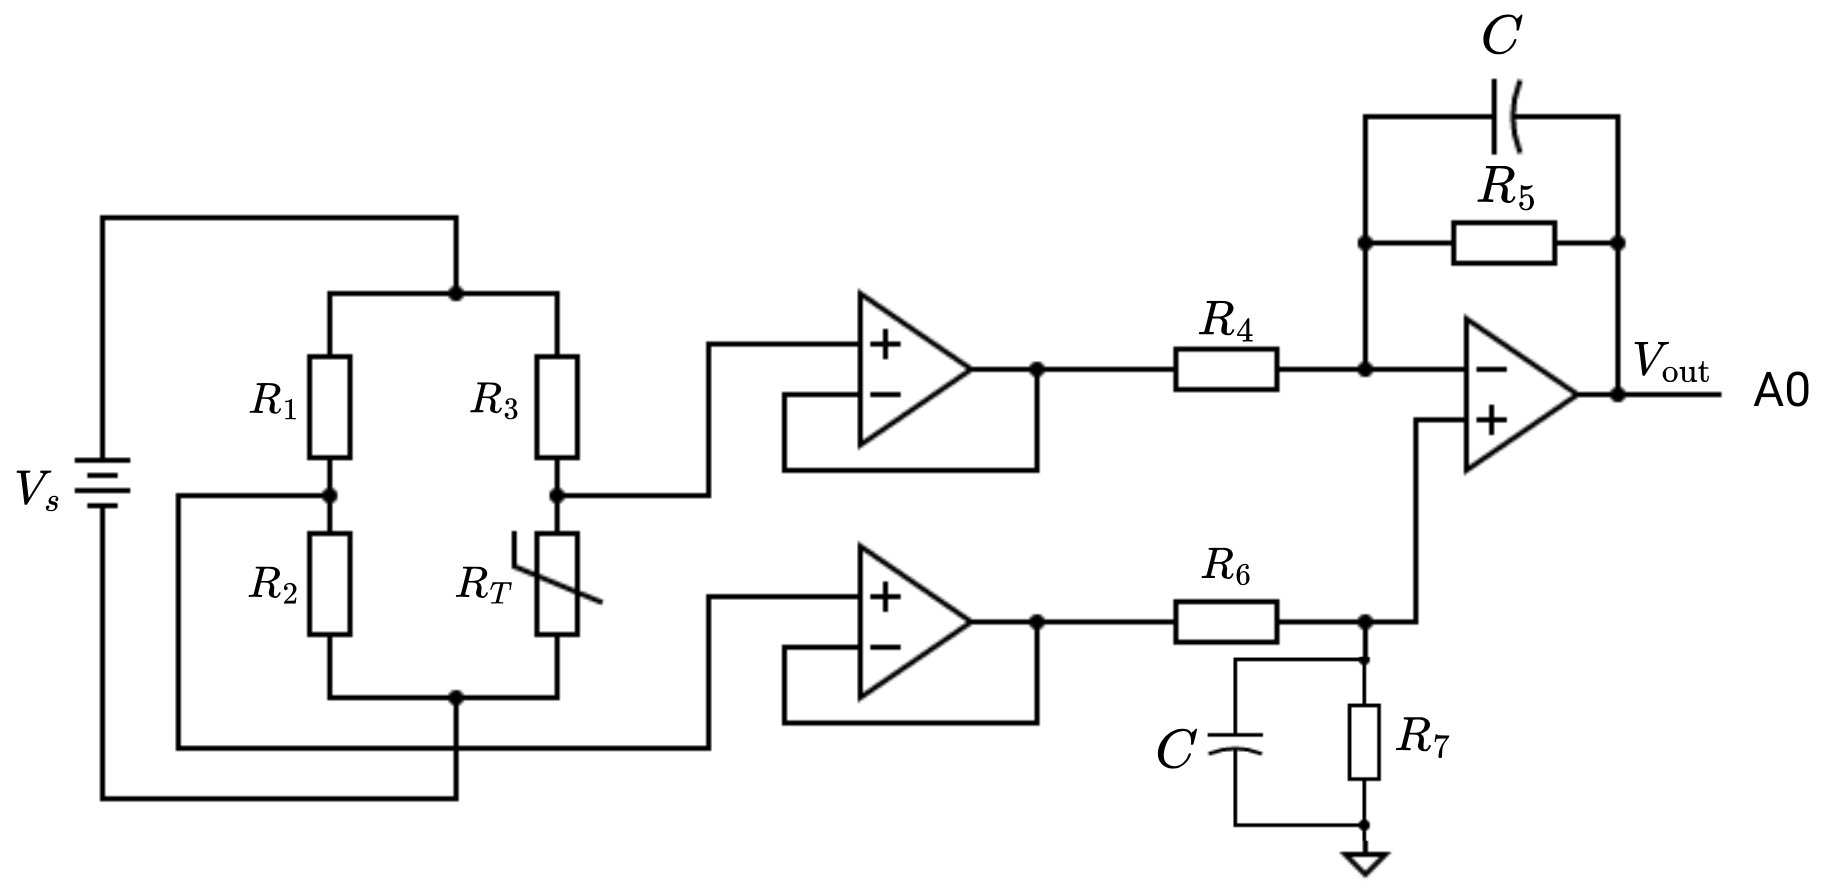
\includegraphics[width=0.7\textwidth]{images/circuit_diagram.png}
    \caption{Connection of the instrumentation circuit output to STM32H743 ADC input (GPIO Pin A0).}
    \label{fig:circuit}
\end{figure}

\section{Circuit Design}
The analog signal from the previously implemented instrumentation circuit is connected to pin A0, which is the built-in ADC channel (ADC1) of the STM32H743VIT6, as shown in Figure~\ref{fig:circuit}.  

\section{Software Configuration and Implementation}

\subsection{Programming Language}

The STM32H743 core board is programmed using the Rust programming language. 
Since the microcontroller uses an ARM Cortex-M7 CPU with FPU~\cite{zephyr}, which uses the Armv7E-M architecture, supporting Thumb/Thumb-2 instruction sets~\cite{arm}, cross-compilation must be configured. 
According to the Rust platform support page~\cite{rust-platform}, the correct target triple is:

\begin{verbatim}
thumbv7em-none-eabihf
\end{verbatim}
This target is added via:
\begin{verbatim}
rustup target add thumbv7em-none-eabihf
\end{verbatim}

\begin{lstlisting}[caption={STM32H743VIT6 Linker Script}, label={lst: linker}]
MEMORY
{
  FLASH  : ORIGIN = 0x08000000, LENGTH = 2048K
  RAM    : ORIGIN = 0x20000000, LENGTH = 128K
}

\end{lstlisting}

A custom memory.x linker script, as shown in Listing~\ref{lst: linker}, was created based on the STM32H743VIT6 
memory map from the reference manual~\cite{ref-manual}. 
Flashing is performed over USB using dfu-util, 
with the appropriate driver installed through Zadig.

\subsection{GPIO}

To provide low-level access to the STM32H743 GPIO peripherals in Rust, 
we developed a gpio module that directly manipulates memory-mapped 
registers using volatile reads and writes.

\paragraph{Enums} 
Two enums were defined to improve readability:
\begin{itemize}
    \item \texttt{GpioPort} --- represents ports A--K.
    \item \texttt{PinMode} --- defines pin modes (\texttt{INPUT}, \texttt{OUTPUT}, 
          \texttt{ALTERNATE}, \texttt{ANALOG}) based on the MODER register encoding.
    \item \texttt{AlternateFunction} --- enumerates AF0--AF15 for use with alternate peripherals.
\end{itemize}

\paragraph{Clock Enabling.}
Before a GPIO port can be used, its peripheral clock must be enabled.  
The function:
\begin{verbatim}
pub unsafe fn rcc_enable_gpio_clock(port: GpioPort)
\end{verbatim}
writes to the \texttt{RCC\_AHB4ENR} register to set the appropriate enable bit.

\paragraph{Pin Mode Configuration.}
The function:
\begin{verbatim}
pub unsafe fn gpio_set_pin_mode(port: GpioPort, pin: u8, mode: PinMode)
\end{verbatim}
modifies the \texttt{MODER} register for the selected port, clearing the 
two mode bits corresponding to the pin and writing the new mode value.

\paragraph{Pin Output Control.}
Two functions are provided:
\begin{itemize}
    \item \texttt{gpio\_set\_pin}: writes to the \texttt{BSRR} register to atomically set or reset a pin.
    \item \texttt{gpio\_toggle\_pin}: reads the \texttt{ODR} register and XORs the bit corresponding to the pin.
\end{itemize}

\paragraph{Alternate Functions.}
The function:
\begin{verbatim}
pub unsafe fn gpio_set_alternate_function(
    port: GpioPort, pin: u8, function: AlternateFunction)
\end{verbatim}
configures the pin’s alternate function by writing to either the 
\texttt{AFRL} (pins 0--7) or \texttt{AFRH} (pins 8--15) register. 

\paragraph{Memory Mapping.}
All register addresses were defined manually:
\begin{itemize}
    \item Base addresses for GPIOA--K were stored in a lookup table (\texttt{GPIO\_BASE\_ADDRS}).
    \item Offsets for MODER, ODR, BSRR, and AFR registers were computed relative to the base.
\end{itemize}

All functions are marked \texttt{unsafe} because they operate 
on raw pointers and memory-mapped I/O, which may cause undefined behavior.

\subsection{Analog to Digital Conversion (ADC)}

\subsubsection{Registers Used}

Each ADC instance is memory-mapped with its own control, configuration, and data registers. In this implementation, we use \textbf{ADC1}, which is mapped at base address \textbf{0x40022000}~\cite[pp.~134]{ref-manual}. The following registers are directly accessed:

\begin{itemize}
    \item \textbf{ISR (Interrupt and Status Register, offset 0x00)}~\cite[pp.~996]{ref-manual}: Provides status flags.
        \begin{itemize}
            \item Bit 0: ADRDY (ADC Ready)
            \item Bit 2: EOC (End of Conversion)
        \end{itemize}
    \item \textbf{CR (Control Register, offset 0x08)}~\cite[pp.~1001]{ref-manual}: Used for power-up, enabling, calibration, and starting conversions.
        \begin{itemize}
            \item Bit 0: ADEN (ADC Enable)
            \item Bit 1: ADDIS (ADC Disable)
            \item Bit 2: ADSTART (Start Regular Conversion)
            \item Bit 28: ADVREGEN (ADC Voltage Regulator Enable)
            \item Bit 29: DEEPPWD (Deep Power Down)
            \item Bit 30: ADCALDIF (Differential Calibration)
            \item Bit 31: ADCAL (Start Calibration)
        \end{itemize}
    \item \textbf{SQR1 (Regular Sequence Register 1, offset 0x30)}~\cite[pp.~1020]{ref-manual}: Defines the channel sequence for conversions.
    \item \textbf{PCSEL (Pre-Channel Selection Register, offset 0x1C)}~\cite[pp.~1018]{ref-manual}: Preselects active input channels.
    \item \textbf{DIFSEL (Differential Selection Register, offset 0xC0)}~\cite[pp.~1031]{ref-manual}: Defines whether inputs are single-ended or differential.
    \item \textbf{DR (Data Register, offset 0x40)}~\cite[pp.~1024]{ref-manual}: Holds the conversion result after EOC is set. For single-ended input mode, the analog voltage to be converted is the
difference between the external voltage $V_{\text{INP[i]}}$ (positive input) and $V_\text{REF-}$ (negative input)~\cite[pp.~924]{ref-manual}, which is \SI{0}{\volt}. The equation for the conversion is
    \begin{equation}
    \label{eq: adc}
        \text{Converted Value} = \text{Max ADC Value} \cdot \frac{V_{\text{out}}}{V_{\text{REF+}}}
    \end{equation}
\end{itemize}

In addition, the common ADC registers are accessed at \textbf{ADC common base address = 0x40022300}:

\begin{itemize}
    \item \textbf{CCR (Common Control Register, offset 0x08)}~\cite[pp.~1035]{ref-manual}: Configures ADC clock mode and prescaler.
    \begin{itemize}
        \item Bit 16-17: CKMODE (ADC Clock Mode)
    \end{itemize}
\end{itemize}

To initialize the clock for ADC, we need to access and modify RCC registers. The following registers are accessed relative to \textbf{base\_addr} of RCC which is \textbf{0x58024400}~\cite[pp.~132]{ref-manual}:

\begin{itemize}
    \item \textbf{AHB1ENR (offset 0xD8)}~\cite[pp.~467]{ref-manual}: Enables the ADC12 peripheral clock.
    \begin{itemize}
        \item Bit 5: ADC12EN (ADC1/2 Peripheral Clocks Enable)
    \end{itemize}
    \item \textbf{D3CCIPR (offset 0x58)}~\cite[pp.~417]{ref-manual}: Selects ADC kernel clock source.
    \begin{itemize}
        \item Bit 16-17: ADCSEL (SAR ADC kernel clock source selection)
    \end{itemize}
\end{itemize}

Finally, $V_{\text{REF}}$ is set by modifying the VREFBUF registers. The following registers are accessed relative \textbf{base\_addr} of VREFBUF which is \textbf{0x58003C00}~\cite[pp.~133]{ref-manual}:

\begin{itemize}

    \item \textbf{CSR (offset 0x00)}~\cite[pp.~297]{ref-manual}: Configures the internal reference buffer and VREF+ selection.
    \begin{itemize}
        \item Bit 4-6: VRS (Voltage reference scale)
        \item Bit 1: HIZ (High impedance mode)
        \item Bit 0: ENVR (Voltage reference buffer mode enable)
    \end{itemize}
\end{itemize}

\subsubsection{Implementation}

\paragraph{Configuring GPIOs}
\begin{itemize}
    \item Enable GPIO port clock via RCC.
    \item Configure the ADC pin (here \textbf{PA0}) to \textbf{Analog mode}~\cite[pp.~88]{ref-manual}.
\end{itemize}

\paragraph{Enabling Clock (\texttt{rcc\_enable\_adc\_clock})}
\begin{itemize}
    \item Enable ADC12 clock by setting \textbf{ADC12EN} in \textbf{RCC\_AHB1ENR}.
    \item Select \textbf{per\_ck} as ADC kernel clock source in \textbf{RCC\_D3CCIPR}.
    \item Set ADC clock mode to synchronous and prescaler (/2) in \textbf{ADC\_CCR}.
\end{itemize}

\paragraph{Power Configuration (\texttt{configure\_pwr})}
\begin{itemize}
    \item Configure \textbf{VREFBUF\_CSR} to enable the internal reference buffer and route it to VREF+.
    \item Select voltage reference scale, set  to \SI{2.5}{\volt} in this implementation.
\end{itemize}

\paragraph{ADC Power-Up (\texttt{adc\_power\_up})}
\begin{itemize}
    \item Clear \textbf{DEEPPWD} in \textbf{ADC\_CR} to exit deep power-down.
    \item Set \textbf{ADVREGEN} to enable the regulator and insert startup delay.
\end{itemize}

\paragraph{Calibration (\texttt{calibrate})}
\begin{itemize}
    \item Ensure ADC is disabled by setting \textbf{ADDIS}.
    \item Configure calibration mode: single-ended (\textbf{ADCALDIF} = 0).
    \item Start calibration by setting \textbf{ADCAL} and wait until it clears.
\end{itemize}

\paragraph{Channel Configuration (\texttt{preselect\_channel}, \texttt{configure\_single\_conversion}, \texttt{set\_diff})}
\begin{itemize}
    \item For ADC1, we use pin A0, which is channel 16~\cite[pp.~68]{datasheet}, so we use \textbf{PCSEL} to preselect channel 16.
    \item Configure \textbf{SQR1} with channel number for first conversion slot.
    \item Ensure channel 16 is single-ended by clearing \textbf{DIFSEL[16]}.
\end{itemize}

\paragraph{Enabling ADC (\texttt{enable})}
\begin{itemize}
    \item Set \textbf{ADEN} in \textbf{CR}.
    \item Wait for \textbf{ADRDY} flag in \textbf{ISR}, then clear it.
\end{itemize}

\paragraph{Starting Conversion (\texttt{start\_conversion})}
\begin{itemize}
    \item Set \textbf{ADSTART} in \textbf{CR}.
\end{itemize}

\begin{lstlisting}[caption={Begin Conversion}, label={lst: adc-begin}]
pub unsafe fn start_conversion(&self) {
    let cr_val = read_volatile(ADC1_CR_ADDR);
    write_volatile(ADC1_CR_ADDR, cr_val | (1 << 2)); // ADSTART = 1
}
\end{lstlisting}

\paragraph{Polling for Completion (\texttt{wait\_for\_conversion})}
\begin{itemize}
    \item Wait for \textbf{EOC} flag in \textbf{ISR}.
\end{itemize}

\begin{lstlisting}[caption={Polling for ADC Completion}, label={lst: adc-complete}]
pub unsafe fn wait_for_conversion(&self) {
    // Wait for End of Conversion (EOC flag in ISR)
    while (read_volatile(ADC1_ISR_ADDR) & (1 << 2)) == 0 {}
}
\end{lstlisting}

\paragraph{Reading Data (\texttt{read\_value})}
\begin{itemize}
    \item Read conversion result from \textbf{DR}.
\end{itemize}

\begin{lstlisting}[caption={Reading Converted Value}, label={lst: adc-read}]
pub unsafe fn read_value(&self) -> u32 {
    read_volatile(ADC1_DR_ADDR)
}
\end{lstlisting}

\subsection{Universal Asynchronous Receiver/Transmitter (UART)}

\subsubsection{Registers Used}

Each UART instance is mapped into memory with its own set of control and data registers. In this implementation, we use USART1 and the following registers are accessed relative to \texttt{base\_addr} of USART1 which is \textbf{0x40011400}~\cite[pp.~134]{ref-manual}:

\begin{itemize}
    \item \textbf{CR1 (Control Register 1, offset 0x00)}~\cite[pp.~2069]{ref-manual}: Used to enable the UART peripheral.
        \begin{itemize}
            \item Bit 0: UE (USART Enable)
            \item Bit 3: TE (Transmitter Enable)
        \end{itemize}
    \item \textbf{BRR (Baud Rate Register, offset 0x0C)}~\cite[pp.~2085]{ref-manual}: Holds the divisor for the baud rate (USARTDIV). With the default oversampling of 16, it is calculated as~\cite[pp.~2036]{ref-manual}
    \begin{equation}
    \label{eq: usart}
        \text{USARTDIV} = \frac{\text{usart\_ker\_ckpres}}{\text{Tx/Rx baud}}
    \end{equation}
    \item \textbf{ISR (Interrupt and Status Register, offset 0x1C)}~\cite[pp.~2088]{ref-manual}: Provides status flags.
        \begin{itemize}
            \item Bit 7: TXE (Transmit Data Register Empty)
        \end{itemize}
    \item \textbf{TDR (Transmit Data Register, offset 0x28)}~\cite[pp.~2101]{ref-manual}: Holds the byte to transmit. Writing here starts the transmission.
\end{itemize}

Additionally, to initialize the clock for USART1, we need to access and modify RCC registers. The following registers are accessed relative to \textbf{base\_addr} of RCC which is \textbf{0x58024400}~\cite[pp.~132]{ref-manual}:

\begin{itemize}
    \item \textbf{APB2ENR (APB2 Clock Register, offset 0xF0)}~\cite[pp.~467]{ref-manual}: Used to enable APB2 peripheral clocks.
        \begin{itemize}
            \item Bit 4: USART1EN (USART1 Peripheral Clocks Enable)
        \end{itemize}
    \item \textbf{D2CFGR (Domain 2 Clock Configuration Register, offset 0x1C)}~\cite[pp.~395]{ref-manual}: Used to configure the domain 2 clock APB prescaler
        \begin{itemize}
            \item Bit 8-10: D2PPRE2 (D2 domain APB2 prescaler)
        \end{itemize}
\end{itemize}

\subsubsection{Implementation}

\paragraph{Configuring GPIOs}
\begin{itemize}
    \item Configure Pin A9 and A10 to be in Alternate Function mode
    \item Configure the alternate function of A9 and A10 to be AF7, which is USART1 TX and RX~\cite[pp.~88]{ref-manual}
\end{itemize}

\paragraph{Enabling Clock (\texttt{rcc\_enable\_uart1\_clock})}
\begin{itemize}
    \item Enable USART1 peripheral clock
    \item Set D2 domain APB2 prescaler to 2
\end{itemize}
All other clock configurations are kept at default value, which means
\begin{itemize}
    \item \textbf{sys\_ck} is \textbf{HSI}, which is \SI{64}{\mega\hertz}~\cite[pp.~1]{datasheet} (RCC\_CFGR~\cite[pp.~390]{ref-manual})
    \item \textbf{sys\_d1cpre\_ck} is \textbf{sys\_ck} (RCC\_D1CFGR~\cite[pp.~393-394]{ref-manual})
    \item \textbf{rcc\_hclk1} is \textbf{sys\_d1cpre\_ck} (RCC\_D1CFGR~\cite[pp.~393-394]{ref-manual})
    \item \textbf{rcc\_pclk2} is \textbf{rcc\_hclk1 / 2} (RCC\_D2CFGR~\cite[pp.~395]{ref-manual})
    \item \textbf{usart\_ker\_ckpres} is \textbf{rcc\_pclk2} (RCC\_D2CCIP2R~\cite[pp. 415-416]{ref-manual}
\end{itemize}
We get that \textbf{usart\_ker\_ckpres} is \SI{32}{\mega\hertz}

\paragraph{Initialization (\texttt{init})}
\begin{itemize}
    \item Calculates the baud rate divisor based on the UART peripheral clock (\texttt{usart\_ker\_ckpres}).
    \item Writes this value to the \textbf{BRR} register.
    \item Enables the UART by setting \textbf{UE} and \textbf{TE} bits in \textbf{CR1}.
\end{itemize}

\begin{lstlisting}[caption={UART Initialization}, label={lst: uart-init}]
let brr_value = usart_ker_ckpres / baudrate;
write_volatile(brr_addr, brr_value);
write_volatile(cr1_addr, cr1 | (1 << 3) | (1 << 0));
\end{lstlisting}

At this point, the UART is active and ready to transmit.

\paragraph{Sending a Byte (\texttt{send\_byte})}
\begin{itemize}
    \item Polls the \textbf{ISR} register until the TXE flag is set, meaning the transmit data register is empty.
    \item Writes the byte into \textbf{TDR}, starting the transfer.
\end{itemize}

\begin{lstlisting}[caption={Sending a Byte}, label={lst: send-byte}]
while (read_volatile(isr_addr) & (1 << 7)) == 0 {}
write_volatile(tdr_addr, byte as u32);
\end{lstlisting}

\paragraph{Sending a String (\texttt{send\_string})}
Iterates through a Rust string's bytes and calls \texttt{send\_byte} on each character:

\begin{lstlisting}[caption={Sending a String}, label={lst: send-string}]
for byte in s.as_bytes() {
    self.send_byte(*byte);
}
\end{lstlisting}

This produces character-by-character UART transmission.

\subsection{Main Program}

\begin{figure}[htbp]
    \centering
    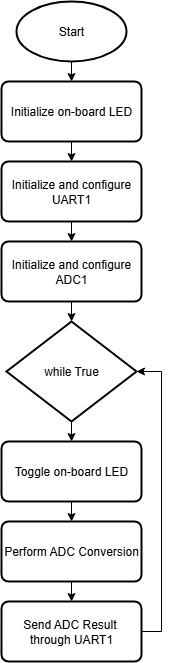
\includegraphics{images/sara-flow.png}
    \caption{Main Program Flowchart}
    \label{fig: flowchart}
\end{figure}

The main program ties together the peripheral abstractions developed in previous modules, namely \texttt{GPIO}, \texttt{UART}, and \texttt{ADC}. It demonstrates peripheral initialization, data acquisition, and communication, while also providing a simple LED toggle as a debugging aid. A flowchart of the main program is shown in Figure~\ref{fig: flowchart}.

\subsubsection{Initialization}

At program startup, we configure the following peripherals:

\begin{itemize}
    \item \textbf{LED (Pin E3)}: Enabled as a general-purpose output for debugging. The LED toggles state on each iteration of the main loop, providing visual confirmation that the program is running correctly.
    \item \textbf{UART1 (Pins A9, A10, Alternate Function AF7)}: Configured with a base address of \texttt{0x40011000}. The GPIO pins are set to alternate function mode AF7 for \texttt{TX} (PA9) and \texttt{RX} (PA10). The peripheral clock is enabled, and the UART is initialized with a baud rate of \SI{115200}{bps}.
    \item \textbf{ADC1 (Pin A0)}: Configured in analog mode. The initialization routine performs the full ADC setup, including power-up, regulator enable, calibration, and channel configuration.
\end{itemize}

\subsubsection{Main Loop}

Once initialization is complete, the program enters its infinite loop:

\begin{enumerate}
    \item Toggle the onboard LED on pin E3.
    \item Start an ADC conversion on channel 0 (PA0).
    \item Poll until the \textbf{End of Conversion (EOC)} flag is set.
    \item Read the resulting 12-bit ADC value from the data register.
    \item Convert the value to its byte representation and transmit the bytes sequentially via UART1.
    \item Delay before repeating the loop.
\end{enumerate}

This process allows us to both visualize the main loop execution (via LED blinking) and validate ADC readings by inspecting UART transmissions.


\section{Demonstration and Verification}

\begin{figure}
    \centering
    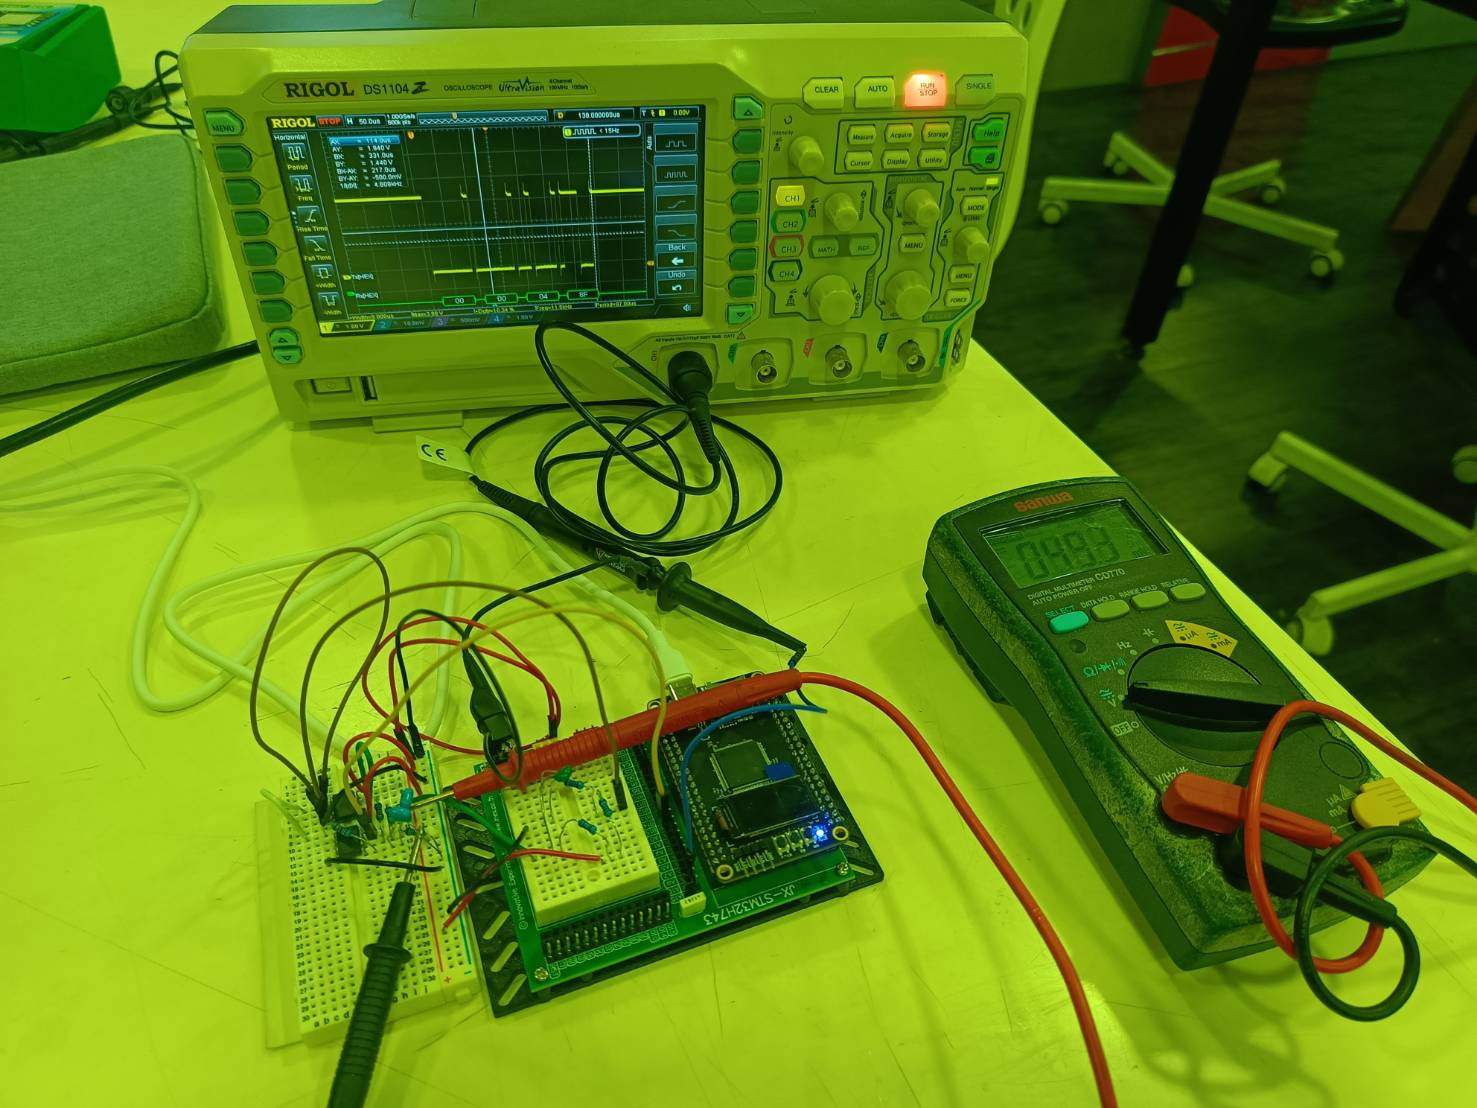
\includegraphics[width=0.8\textwidth]{images/setup.jpg}
    \caption{Overall experimental setup with STM32 board, oscilloscope, and multimeter.}
    \label{fig:setup}
\end{figure}

\begin{figure}
    \centering
    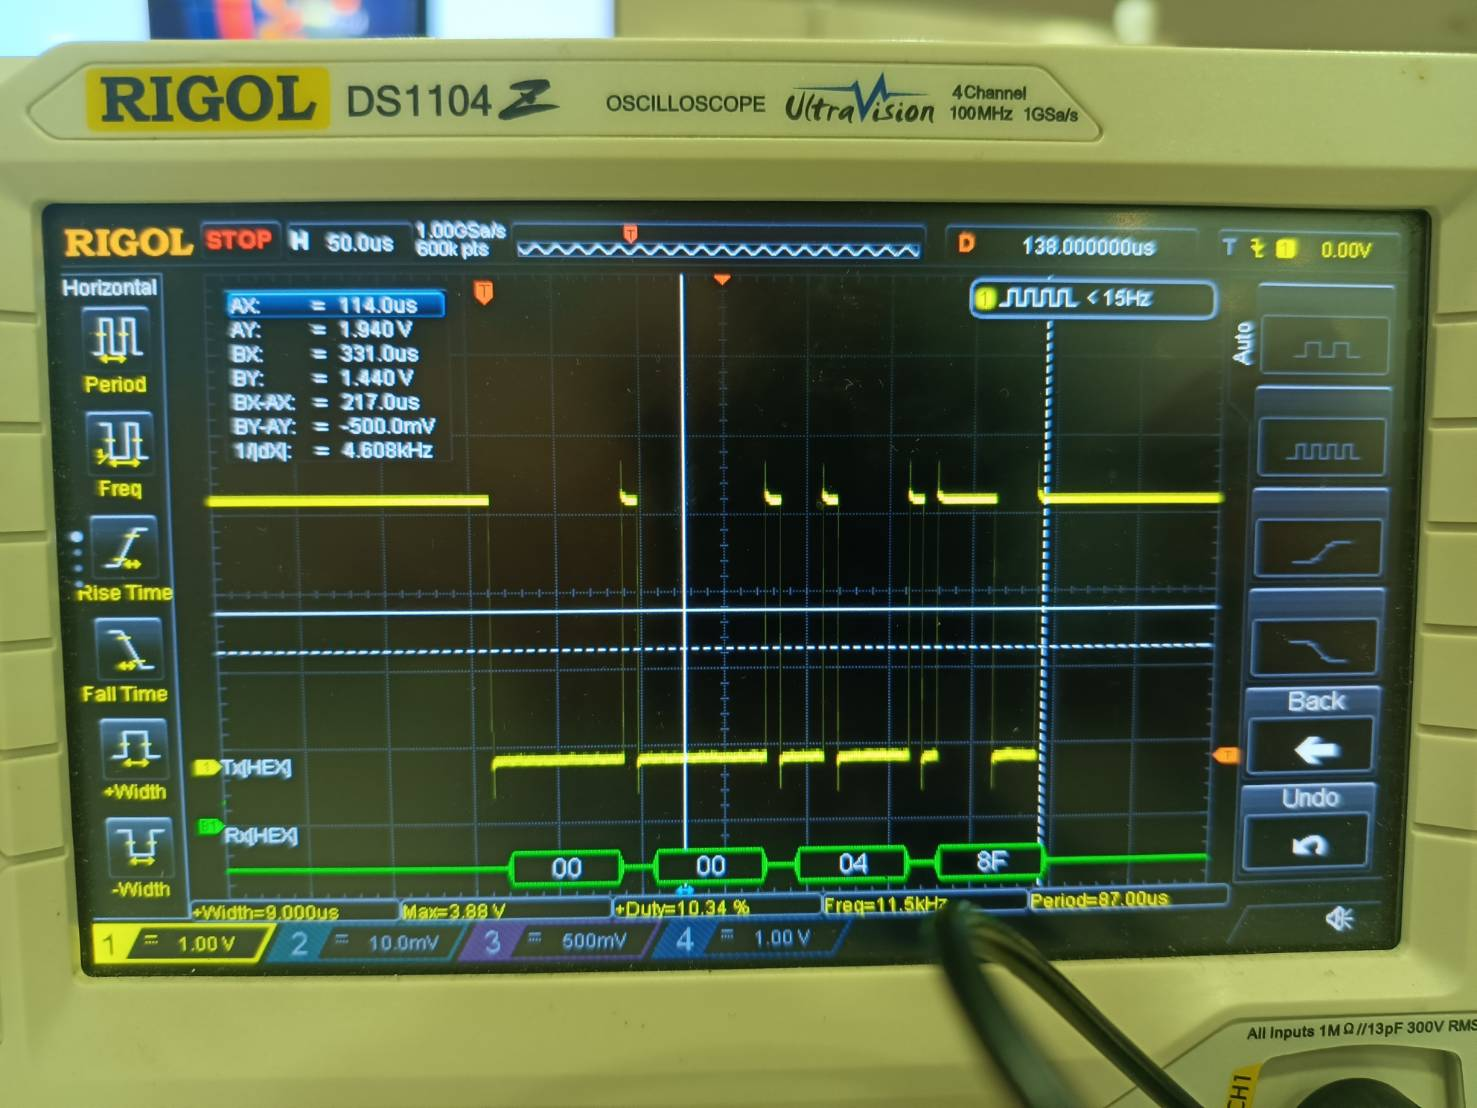
\includegraphics[width=0.8\textwidth]{images/oscilloscope.jpg}
    \caption{Decoded UART transmission displayed on the Rigol DS1104Z oscilloscope.}
    \label{fig:oscilloscope}
\end{figure}

\begin{figure}
    \centering
    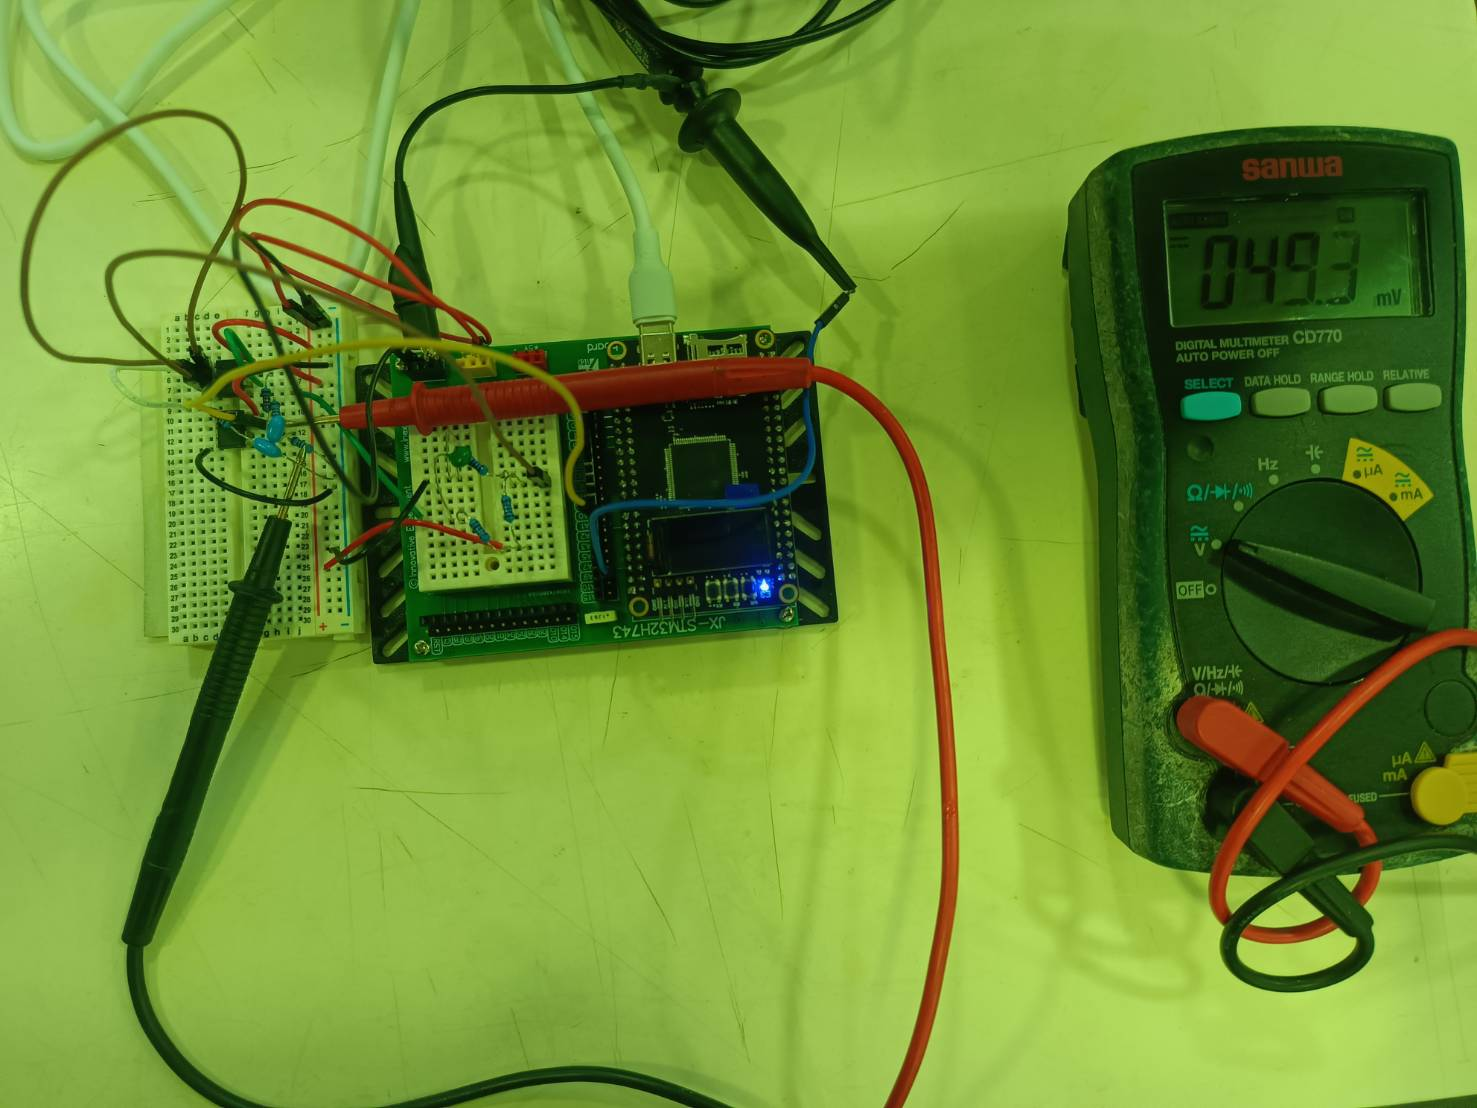
\includegraphics[width=0.8\textwidth]{images/multimeter.jpg}
    \caption{Voltage measurement of the transducer output using Sanwa CD770 Digital Multimeter.}
    \label{fig:multimeter}
\end{figure}

To demonstrate and verify the operation of the implemented system, the analog signal from the previously implemented instrumentation circuit is connected to pin A0, as shown in Figure~\ref{fig:circuit}, which corresponds to the ADC1\_IN16 input channel of the STM32H743 microcontroller. The main program samples the analog signal at A0 and converts it using the ADC. The conversion result is then transmitted via UART1 on pin A9 (TX). 

To observe and verify the digital values, we connect a Rigol DS1104Z oscilloscope to pin A9 and use its UART decode function and compare the value to the reading from a Sanwa CD770 Digital Multimeter connected directly to the analog output of the instrumentation circuit, as shown in Figure~\ref{fig:setup}.

We collected 20 readings from the oscilloscope, one of which is shown in Figure~\ref{fig:oscilloscope}, each corresponding to the ADC conversion result transmitted via UART. The raw ADC values $N$ were converted into voltages using the ADC resolution relation given from solving~\eqref{eq: adc}

\begin{equation*}
    V_{\text{out}} = V_{\text{REF+}} \cdot \frac{\text{Converted Value}}{\text{Max ADC Value}}
\end{equation*}

where $V_{\text{ref}} = \SI{2.5}{\volt}$ and $\text{Max ADC Value} = 2^{16}-1 = 65535$. The converted values were then averaged, and the standard deviation was calculated.

The decoded UART values correspond to an average voltage of

\[
    V_{\text{out}} \approx \SI{43.05}{\milli\volt}
\]

The multimeter measurement, as shown in Figure~\ref{fig:multimeter}, gave a value of

\[
    V_{\text{dmm}} = \SI{49.3}{\milli\volt} \pm \SI{0.4}{\milli\volt}
\]  

From the measurements, we can calculate the error to be

% \begin{align*}
%     \text{Error} & = |{\frac{V_{\text{out}} - V_{\text{dmm}}}{V_{\text{dmm}}}}| \times 100 \\
%     & = |\frac{\SI{43.05}{\milli\volt} - \SI{49.3}{\milli\volt}}{\SI{49.3}{\milli\volt}}| \times 100 \\
%     & \approx 12.68 \percent 
% \end{align*}

\begin{align*}
    \text{Error} & = \left|\frac{V_{\text{out}} - V_{\text{dmm}}}{V_{\text{dmm}}}\right| \times 100 \\
    & = \left|\frac{\SI{43.05}{\milli\volt} - \SI{49.3}{\milli\volt}}{\SI{49.3}{\milli\volt}}\right| \times 100 \\
    & \approx 12.68 \%
\end{align*}


\section{Conclusion}
The STM32H743 successfully performs analog-to-digital conversion of the temperature sensor output and transmits the measured values via UART. The implementation includes:
\begin{itemize}
    \item Proper configuration of the ADC peripheral
    \item UART transmission for monitoring
\end{itemize}

\newpage
\bibliographystyle{IEEEtran}
\bibliography{ref}

\end{document}
